\documentclass[1p]{elsarticle_modified}
%\bibliographystyle{elsarticle-num}

%\usepackage[colorlinks]{hyperref}
%\usepackage{abbrmath_seonhwa} %\Abb, \Ascr, \Acal ,\Abf, \Afrak
\usepackage{amsfonts}
\usepackage{amssymb}
\usepackage{amsmath}
\usepackage{amsthm}
\usepackage{scalefnt}
\usepackage{amsbsy}
\usepackage{kotex}
\usepackage{caption}
\usepackage{subfig}
\usepackage{color}
\usepackage{graphicx}
\usepackage{xcolor} %% white, black, red, green, blue, cyan, magenta, yellow
\usepackage{float}
\usepackage{setspace}
\usepackage{hyperref}

\usepackage{tikz}
\usetikzlibrary{arrows}

\usepackage{multirow}
\usepackage{array} % fixed length table
\usepackage{hhline}

%%%%%%%%%%%%%%%%%%%%%
\makeatletter
\renewcommand*\env@matrix[1][\arraystretch]{%
	\edef\arraystretch{#1}%
	\hskip -\arraycolsep
	\let\@ifnextchar\new@ifnextchar
	\array{*\c@MaxMatrixCols c}}
\makeatother %https://tex.stackexchange.com/questions/14071/how-can-i-increase-the-line-spacing-in-a-matrix
%%%%%%%%%%%%%%%

\usepackage[normalem]{ulem}

\newcommand{\msout}[1]{\ifmmode\text{\sout{\ensuremath{#1}}}\else\sout{#1}\fi}
%SOURCE: \msout is \stkout macro in https://tex.stackexchange.com/questions/20609/strikeout-in-math-mode

\newcommand{\cancel}[1]{
	\ifmmode
	{\color{red}\msout{#1}}
	\else
	{\color{red}\sout{#1}}
	\fi
}

\newcommand{\add}[1]{
	{\color{blue}\uwave{#1}}
}

\newcommand{\replace}[2]{
	\ifmmode
	{\color{red}\msout{#1}}{\color{blue}\uwave{#2}}
	\else
	{\color{red}\sout{#1}}{\color{blue}\uwave{#2}}
	\fi
}

\newcommand{\Sol}{\mathcal{S}} %segment
\newcommand{\D}{D} %diagram
\newcommand{\A}{\mathcal{A}} %arc


%%%%%%%%%%%%%%%%%%%%%%%%%%%%%5 test

\def\sl{\operatorname{\textup{SL}}(2,\Cbb)}
\def\psl{\operatorname{\textup{PSL}}(2,\Cbb)}
\def\quan{\mkern 1mu \triangleright \mkern 1mu}

\theoremstyle{definition}
\newtheorem{thm}{Theorem}[section]
\newtheorem{prop}[thm]{Proposition}
\newtheorem{lem}[thm]{Lemma}
\newtheorem{ques}[thm]{Question}
\newtheorem{cor}[thm]{Corollary}
\newtheorem{defn}[thm]{Definition}
\newtheorem{exam}[thm]{Example}
\newtheorem{rmk}[thm]{Remark}
\newtheorem{alg}[thm]{Algorithm}

\newcommand{\I}{\sqrt{-1}}
\begin{document}

%\begin{frontmatter}
%
%\title{Boundary parabolic representations of knots up to 8 crossings}
%
%%% Group authors per affiliation:
%\author{Yunhi Cho} 
%\address{Department of Mathematics, University of Seoul, Seoul, Korea}
%\ead{yhcho@uos.ac.kr}
%
%
%\author{Seonhwa Kim} %\fnref{s_kim}}
%\address{Center for Geometry and Physics, Institute for Basic Science, Pohang, 37673, Korea}
%\ead{ryeona17@ibs.re.kr}
%
%\author{Hyuk Kim}
%\address{Department of Mathematical Sciences, Seoul National University, Seoul 08826, Korea}
%\ead{hyukkim@snu.ac.kr}
%
%\author{Seokbeom Yoon}
%\address{Department of Mathematical Sciences, Seoul National University, Seoul, 08826,  Korea}
%\ead{sbyoon15@snu.ac.kr}
%
%\begin{abstract}
%We find all boundary parabolic representation of knots up to 8 crossings.
%
%\end{abstract}
%\begin{keyword}
%    \MSC[2010] 57M25 
%\end{keyword}
%
%\end{frontmatter}

%\linenumbers
%\tableofcontents
%
\newcommand\colored[1]{\textcolor{white}{\rule[-0.35ex]{0.8em}{1.4ex}}\kern-0.8em\color{red} #1}%
%\newcommand\colored[1]{\textcolor{white}{ #1}\kern-2.17ex	\textcolor{white}{ #1}\kern-1.81ex	\textcolor{white}{ #1}\kern-2.15ex\color{red}#1	}

{\Large $\underline{12a_{0772}~(K12a_{0772})}$}

\setlength{\tabcolsep}{10pt}
\renewcommand{\arraystretch}{1.6}
\vspace{1cm}\begin{tabular}{m{100pt}>{\centering\arraybackslash}m{274pt}}
\multirow{5}{120pt}{
	\centering
	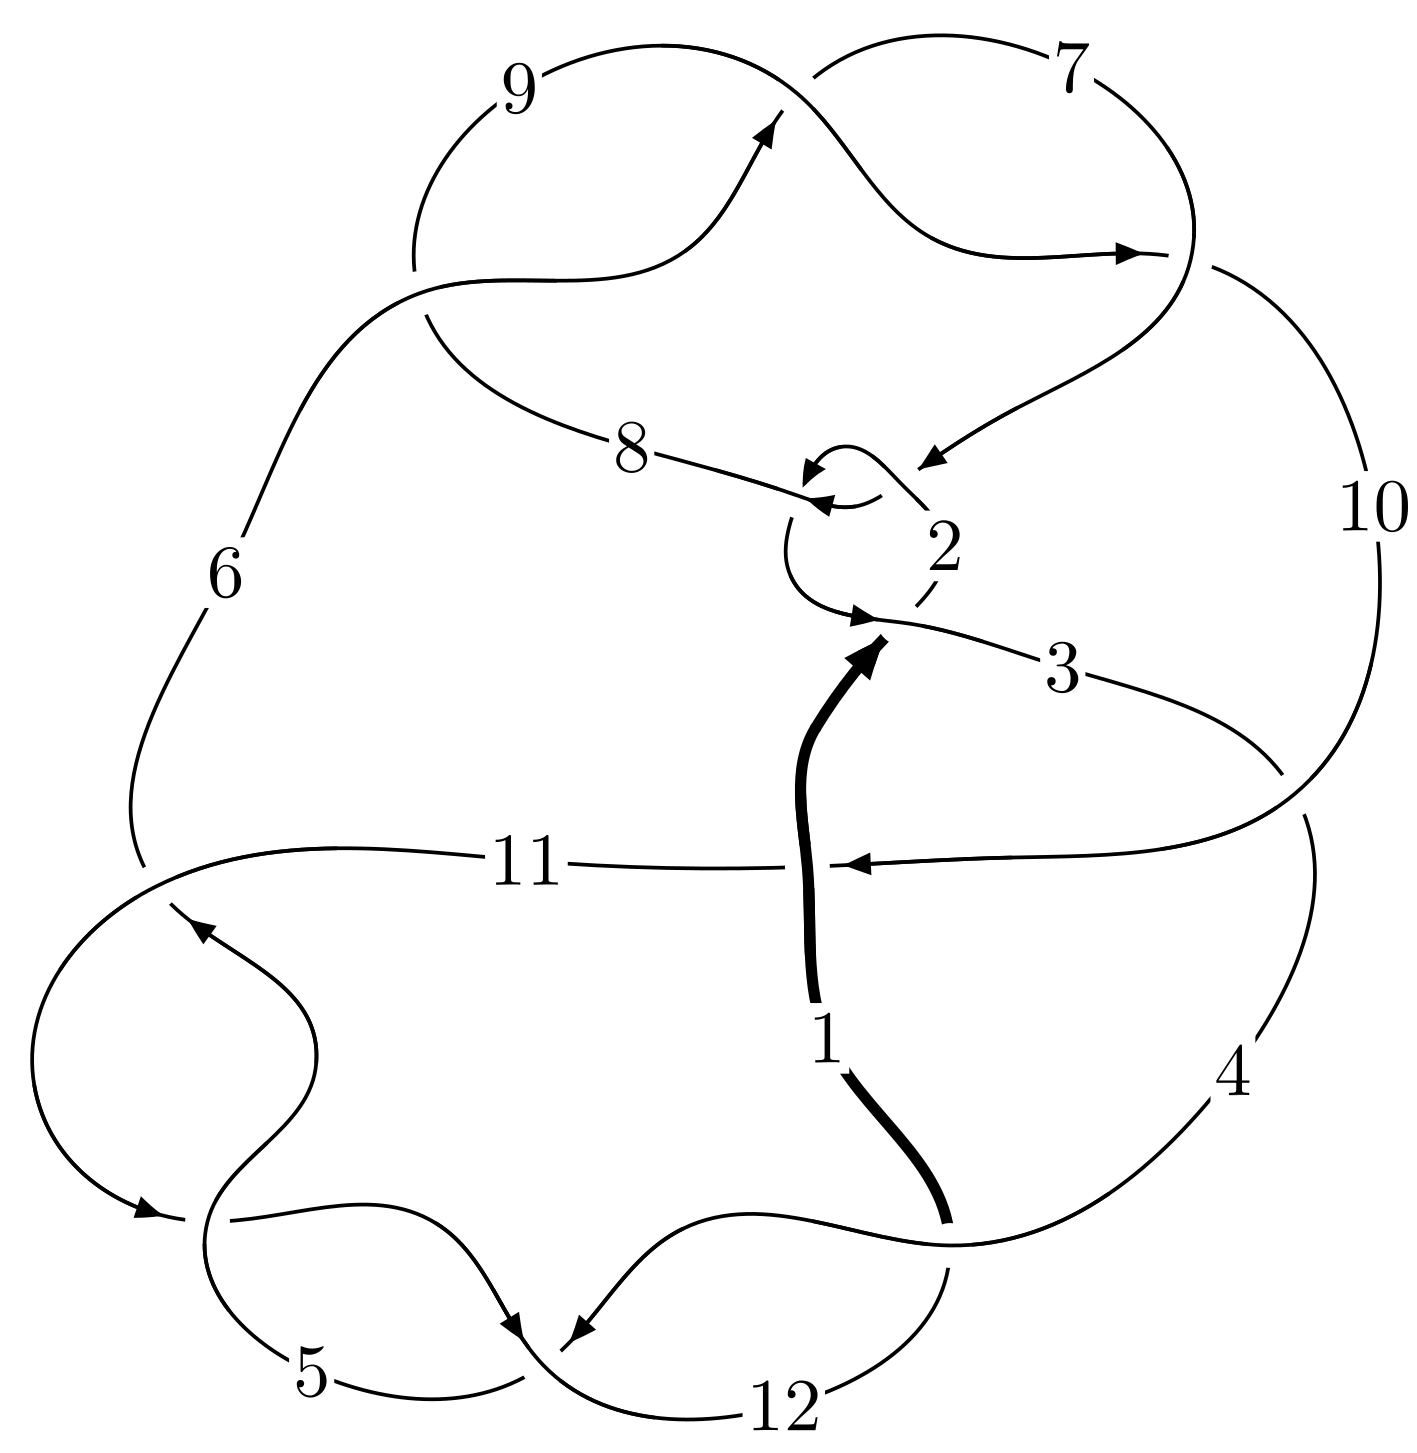
\includegraphics[width=112pt]{../../../GIT/diagram.site/Diagrams/png/1573_12a_0772.png}\\
\ \ \ A knot diagram\footnotemark}&
\allowdisplaybreaks
\textbf{Linearized knot diagam} \\
\cline{2-2}
 &
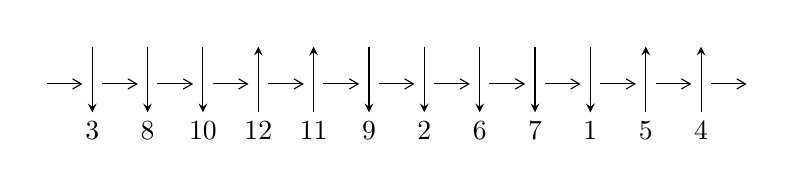
\begin{tikzpicture}[x=20pt, y=17pt]
	% nodes
	\node (C0) at (0, 0) {};
	\node (C1) at (1, 0) {};
	\node (C1U) at (1, +1) {};
	\node (C1D) at (1, -1) {3};

	\node (C2) at (2, 0) {};
	\node (C2U) at (2, +1) {};
	\node (C2D) at (2, -1) {8};

	\node (C3) at (3, 0) {};
	\node (C3U) at (3, +1) {};
	\node (C3D) at (3, -1) {10};

	\node (C4) at (4, 0) {};
	\node (C4U) at (4, +1) {};
	\node (C4D) at (4, -1) {12};

	\node (C5) at (5, 0) {};
	\node (C5U) at (5, +1) {};
	\node (C5D) at (5, -1) {11};

	\node (C6) at (6, 0) {};
	\node (C6U) at (6, +1) {};
	\node (C6D) at (6, -1) {9};

	\node (C7) at (7, 0) {};
	\node (C7U) at (7, +1) {};
	\node (C7D) at (7, -1) {2};

	\node (C8) at (8, 0) {};
	\node (C8U) at (8, +1) {};
	\node (C8D) at (8, -1) {6};

	\node (C9) at (9, 0) {};
	\node (C9U) at (9, +1) {};
	\node (C9D) at (9, -1) {7};

	\node (C10) at (10, 0) {};
	\node (C10U) at (10, +1) {};
	\node (C10D) at (10, -1) {1};

	\node (C11) at (11, 0) {};
	\node (C11U) at (11, +1) {};
	\node (C11D) at (11, -1) {5};

	\node (C12) at (12, 0) {};
	\node (C12U) at (12, +1) {};
	\node (C12D) at (12, -1) {4};
	\node (C13) at (13, 0) {};

	% arrows
	\draw[->,>={angle 60}]
	(C0) edge (C1) (C1) edge (C2) (C2) edge (C3) (C3) edge (C4) (C4) edge (C5) (C5) edge (C6) (C6) edge (C7) (C7) edge (C8) (C8) edge (C9) (C9) edge (C10) (C10) edge (C11) (C11) edge (C12) (C12) edge (C13) ;	\draw[->,>=stealth]
	(C1U) edge (C1D) (C2U) edge (C2D) (C3U) edge (C3D) (C4D) edge (C4U) (C5D) edge (C5U) (C6U) edge (C6D) (C7U) edge (C7D) (C8U) edge (C8D) (C9U) edge (C9D) (C10U) edge (C10D) (C11D) edge (C11U) (C12D) edge (C12U) ;
	\end{tikzpicture} \\
\hhline{~~} \\& 
\textbf{Solving Sequence} \\ \cline{2-2} 
 &
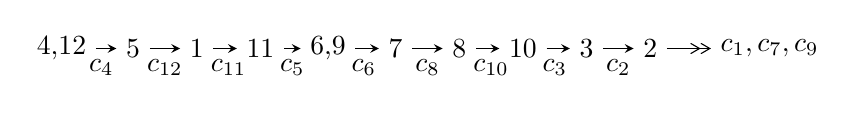
\begin{tikzpicture}[x=23pt, y=7pt]
	% node
	\node (A0) at (-1/8, 0) {4,12};
	\node (A1) at (1, 0) {5};
	\node (A2) at (2, 0) {1};
	\node (A3) at (3, 0) {11};
	\node (A4) at (65/16, 0) {6,9};
	\node (A5) at (41/8, 0) {7};
	\node (A6) at (49/8, 0) {8};
	\node (A7) at (57/8, 0) {10};
	\node (A8) at (65/8, 0) {3};
	\node (A9) at (73/8, 0) {2};
	\node (C1) at (1/2, -1) {$c_{4}$};
	\node (C2) at (3/2, -1) {$c_{12}$};
	\node (C3) at (5/2, -1) {$c_{11}$};
	\node (C4) at (7/2, -1) {$c_{5}$};
	\node (C5) at (37/8, -1) {$c_{6}$};
	\node (C6) at (45/8, -1) {$c_{8}$};
	\node (C7) at (53/8, -1) {$c_{10}$};
	\node (C8) at (61/8, -1) {$c_{3}$};
	\node (C9) at (69/8, -1) {$c_{2}$};
	\node (A10) at (11, 0) {$c_{1},c_{7},c_{9}$};

	% edge
	\draw[->,>=stealth]	
	(A0) edge (A1) (A1) edge (A2) (A2) edge (A3) (A3) edge (A4) (A4) edge (A5) (A5) edge (A6) (A6) edge (A7) (A7) edge (A8) (A8) edge (A9) ;
	\draw[->>,>={angle 60}]	
	(A9) edge (A10);
\end{tikzpicture} \\ 

\end{tabular} \\

\footnotetext{
The image of knot diagram is generated by the software ``\textbf{Draw programme}" developed by Andrew Bartholomew(\url{http://www.layer8.co.uk/maths/draw/index.htm\#Running-draw}), where we modified some parts for our purpose(\url{https://github.com/CATsTAILs/LinksPainter}).
}\phantom \\ \newline 
\centering \textbf{Ideals for irreducible components\footnotemark of $X_{\text{par}}$} 
 
\begin{align*}
I^u_{1}&=\langle 
u^{67}+2 u^{66}+\cdots+b+1,\;u^{67}+2 u^{66}+\cdots+a+2,\;u^{68}+2 u^{67}+\cdots+6 u+1\rangle \\
I^u_{2}&=\langle 
b,\;u^3+a+2 u,\;u^4- u^3+3 u^2-2 u+1\rangle \\
\\
\end{align*}
\raggedright * 2 irreducible components of $\dim_{\mathbb{C}}=0$, with total 72 representations.\\
\footnotetext{All coefficients of polynomials are rational numbers. But the coefficients are sometimes approximated in decimal forms when there is not enough margin.}
\newpage
\renewcommand{\arraystretch}{1}
\centering \section*{I. $I^u_{1}= \langle u^{67}+2 u^{66}+\cdots+b+1,\;u^{67}+2 u^{66}+\cdots+a+2,\;u^{68}+2 u^{67}+\cdots+6 u+1 \rangle$}
\flushleft \textbf{(i) Arc colorings}\\
\begin{tabular}{m{7pt} m{180pt} m{7pt} m{180pt} }
\flushright $a_{4}=$&$\begin{pmatrix}1\\0\end{pmatrix}$ \\
\flushright $a_{12}=$&$\begin{pmatrix}0\\u\end{pmatrix}$ \\
\flushright $a_{5}=$&$\begin{pmatrix}1\\- u^2\end{pmatrix}$ \\
\flushright $a_{1}=$&$\begin{pmatrix}u\\u\end{pmatrix}$ \\
\flushright $a_{11}=$&$\begin{pmatrix}- u\\u^3+u\end{pmatrix}$ \\
\flushright $a_{6}=$&$\begin{pmatrix}u^2+1\\- u^4-2 u^2\end{pmatrix}$ \\
\flushright $a_{9}=$&$\begin{pmatrix}- u^{67}-2 u^{66}+\cdots-6 u-2\\- u^{67}-2 u^{66}+\cdots-4 u-1\end{pmatrix}$ \\
\flushright $a_{7}=$&$\begin{pmatrix}u^{67}+u^{66}+\cdots+2 u+2\\- u^{41}-23 u^{39}+\cdots-2 u^2- u\end{pmatrix}$ \\
\flushright $a_{8}=$&$\begin{pmatrix}- u^{67}-3 u^{66}+\cdots-8 u-3\\-2 u^{67}-4 u^{66}+\cdots-10 u-2\end{pmatrix}$ \\
\flushright $a_{10}=$&$\begin{pmatrix}u^5+2 u^3- u\\u^5+3 u^3+u\end{pmatrix}$ \\
\flushright $a_{3}=$&$\begin{pmatrix}- u^{10}-5 u^8-6 u^6+u^4+u^2+1\\- u^{10}-6 u^8-11 u^6-6 u^4- u^2\end{pmatrix}$ \\
\flushright $a_{2}=$&$\begin{pmatrix}u^{19}+10 u^{17}+38 u^{15}+66 u^{13}+47 u^{11}+4 u^9-8 u^7-10 u^5-3 u^3\\u^{19}+11 u^{17}+48 u^{15}+105 u^{13}+121 u^{11}+75 u^9+30 u^7+8 u^5+u^3+u\end{pmatrix}$\\&\end{tabular}
\flushleft \textbf{(ii) Obstruction class $= -1$}\\~\\
\flushleft \textbf{(iii) Cusp Shapes $= u^{67}+2 u^{66}+\cdots- u-9$}\\~\\
\newpage\renewcommand{\arraystretch}{1}
\flushleft \textbf{(iv) u-Polynomials at the component}\newline \\
\begin{tabular}{m{50pt}|m{274pt}}
Crossings & \hspace{64pt}u-Polynomials at each crossing \\
\hline $$\begin{aligned}c_{1}\end{aligned}$$&$\begin{aligned}
&u^{68}+27 u^{67}+\cdots+1344 u+256
\end{aligned}$\\
\hline $$\begin{aligned}c_{2},c_{7}\end{aligned}$$&$\begin{aligned}
&u^{68}+u^{67}+\cdots-40 u-16
\end{aligned}$\\
\hline $$\begin{aligned}c_{3}\end{aligned}$$&$\begin{aligned}
&u^{68}+2 u^{67}+\cdots+5322 u+1049
\end{aligned}$\\
\hline $$\begin{aligned}c_{4},c_{5},c_{11}\\c_{12}\end{aligned}$$&$\begin{aligned}
&u^{68}+2 u^{67}+\cdots+6 u+1
\end{aligned}$\\
\hline $$\begin{aligned}c_{6},c_{8},c_{9}\end{aligned}$$&$\begin{aligned}
&u^{68}-5 u^{67}+\cdots+6 u-1
\end{aligned}$\\
\hline $$\begin{aligned}c_{10}\end{aligned}$$&$\begin{aligned}
&u^{68}-18 u^{67}+\cdots-1008 u+49
\end{aligned}$\\
\hline
\end{tabular}\\~\\
\newpage\renewcommand{\arraystretch}{1}
\flushleft \textbf{(v) Riley Polynomials at the component}\newline \\
\begin{tabular}{m{50pt}|m{274pt}}
Crossings & \hspace{64pt}Riley Polynomials at each crossing \\
\hline $$\begin{aligned}c_{1}\end{aligned}$$&$\begin{aligned}
&y^{68}+21 y^{67}+\cdots-1232896 y+65536
\end{aligned}$\\
\hline $$\begin{aligned}c_{2},c_{7}\end{aligned}$$&$\begin{aligned}
&y^{68}-27 y^{67}+\cdots-1344 y+256
\end{aligned}$\\
\hline $$\begin{aligned}c_{3}\end{aligned}$$&$\begin{aligned}
&y^{68}-18 y^{67}+\cdots-32379118 y+1100401
\end{aligned}$\\
\hline $$\begin{aligned}c_{4},c_{5},c_{11}\\c_{12}\end{aligned}$$&$\begin{aligned}
&y^{68}+78 y^{67}+\cdots-6 y+1
\end{aligned}$\\
\hline $$\begin{aligned}c_{6},c_{8},c_{9}\end{aligned}$$&$\begin{aligned}
&y^{68}-59 y^{67}+\cdots-12 y+1
\end{aligned}$\\
\hline $$\begin{aligned}c_{10}\end{aligned}$$&$\begin{aligned}
&y^{68}-6 y^{67}+\cdots-75166 y+2401
\end{aligned}$\\
\hline
\end{tabular}\\~\\
\newpage\flushleft \textbf{(vi) Complex Volumes and Cusp Shapes}
$$\begin{array}{c|c|c}  
\text{Solutions to }I^u_{1}& \I (\text{vol} + \sqrt{-1}CS) & \text{Cusp shape}\\
 \hline 
\begin{aligned}
u &= -0.197347 + 0.873475 I \\
a &= -1.89430 + 0.94588 I \\
b &= -1.68578 - 0.87347 I\end{aligned}
 & -6.76573 + 5.38396 I & -12.62780 + 0. I\phantom{ +0.000000I} \\ \hline\begin{aligned}
u &= -0.197347 - 0.873475 I \\
a &= -1.89430 - 0.94588 I \\
b &= -1.68578 + 0.87347 I\end{aligned}
 & -6.76573 - 5.38396 I & -12.62780 + 0. I\phantom{ +0.000000I} \\ \hline\begin{aligned}
u &= -0.400919 + 0.776860 I \\
a &= -1.74029 + 2.14685 I \\
b &= -2.54116 - 0.78686 I\end{aligned}
 & -10.07420 - 3.27035 I & -14.2388 + 4.5595 I \\ \hline\begin{aligned}
u &= -0.400919 - 0.776860 I \\
a &= -1.74029 - 2.14685 I \\
b &= -2.54116 + 0.78686 I\end{aligned}
 & -10.07420 + 3.27035 I & -14.2388 - 4.5595 I \\ \hline\begin{aligned}
u &= -0.516725 + 0.700827 I \\
a &= -0.69973 + 2.63609 I \\
b &= -2.80366 - 0.05209 I\end{aligned}
 & -4.70584 - 11.85590 I & -9.20800 + 9.67141 I \\ \hline\begin{aligned}
u &= -0.516725 - 0.700827 I \\
a &= -0.69973 - 2.63609 I \\
b &= -2.80366 + 0.05209 I\end{aligned}
 & -4.70584 + 11.85590 I & -9.20800 - 9.67141 I \\ \hline\begin{aligned}
u &= -0.495876 + 0.679831 I \\
a &= \phantom{-}0.682404 - 0.604436 I \\
b &= \phantom{-}1.120320 + 0.179470 I\end{aligned}
 & \phantom{-}0.39345 - 7.62900 I & -5.28637 + 9.02700 I \\ \hline\begin{aligned}
u &= -0.495876 - 0.679831 I \\
a &= \phantom{-}0.682404 + 0.604436 I \\
b &= \phantom{-}1.120320 - 0.179470 I\end{aligned}
 & \phantom{-}0.39345 + 7.62900 I & -5.28637 - 9.02700 I \\ \hline\begin{aligned}
u &= \phantom{-}0.474084 + 0.680555 I \\
a &= \phantom{-}0.96634 + 3.09061 I \\
b &= \phantom{-}3.15400 - 0.19444 I\end{aligned}
 & -2.72085 + 5.66166 I & -8.20435 - 6.61637 I \\ \hline\begin{aligned}
u &= \phantom{-}0.474084 - 0.680555 I \\
a &= \phantom{-}0.96634 - 3.09061 I \\
b &= \phantom{-}3.15400 + 0.19444 I\end{aligned}
 & -2.72085 - 5.66166 I & -8.20435 + 6.61637 I\\
 \hline 
 \end{array}$$\newpage$$\begin{array}{c|c|c}  
\text{Solutions to }I^u_{1}& \I (\text{vol} + \sqrt{-1}CS) & \text{Cusp shape}\\
 \hline 
\begin{aligned}
u &= -0.450615 + 0.661293 I \\
a &= \phantom{-}0.423151 - 0.930817 I \\
b &= \phantom{-}0.078954 + 0.208633 I\end{aligned}
 & -1.99409 - 3.06832 I & -9.13804 + 6.00596 I \\ \hline\begin{aligned}
u &= -0.450615 - 0.661293 I \\
a &= \phantom{-}0.423151 + 0.930817 I \\
b &= \phantom{-}0.078954 - 0.208633 I\end{aligned}
 & -1.99409 + 3.06832 I & -9.13804 - 6.00596 I \\ \hline\begin{aligned}
u &= \phantom{-}0.481088 + 0.620510 I \\
a &= -0.751512 - 0.690976 I \\
b &= -1.050000 + 0.375121 I\end{aligned}
 & \phantom{-}1.64508 + 2.45629 I & -1.94498 - 3.97918 I \\ \hline\begin{aligned}
u &= \phantom{-}0.481088 - 0.620510 I \\
a &= -0.751512 + 0.690976 I \\
b &= -1.050000 - 0.375121 I\end{aligned}
 & \phantom{-}1.64508 - 2.45629 I & -1.94498 + 3.97918 I \\ \hline\begin{aligned}
u &= -0.170138 + 0.764448 I \\
a &= \phantom{-}0.198071 - 0.774648 I \\
b &= \phantom{-}0.091517 + 0.187313 I\end{aligned}
 & -1.56053 + 1.82446 I & -9.18170 - 2.54653 I \\ \hline\begin{aligned}
u &= -0.170138 - 0.764448 I \\
a &= \phantom{-}0.198071 + 0.774648 I \\
b &= \phantom{-}0.091517 - 0.187313 I\end{aligned}
 & -1.56053 - 1.82446 I & -9.18170 + 2.54653 I \\ \hline\begin{aligned}
u &= \phantom{-}0.532445 + 0.564325 I \\
a &= -0.388234 - 1.011420 I \\
b &= \phantom{-}0.050264 + 0.201909 I\end{aligned}
 & -2.03493 - 0.49893 I & -8.07852 - 0.03154 I \\ \hline\begin{aligned}
u &= \phantom{-}0.532445 - 0.564325 I \\
a &= -0.388234 + 1.011420 I \\
b &= \phantom{-}0.050264 - 0.201909 I\end{aligned}
 & -2.03493 + 0.49893 I & -8.07852 + 0.03154 I \\ \hline\begin{aligned}
u &= \phantom{-}0.243977 + 0.727217 I \\
a &= \phantom{-}2.80371 + 1.23958 I \\
b &= \phantom{-}1.88635 - 1.53609 I\end{aligned}
 & -4.18607 - 0.03385 I & -11.57789 - 1.81848 I \\ \hline\begin{aligned}
u &= \phantom{-}0.243977 - 0.727217 I \\
a &= \phantom{-}2.80371 - 1.23958 I \\
b &= \phantom{-}1.88635 + 1.53609 I\end{aligned}
 & -4.18607 + 0.03385 I & -11.57789 + 1.81848 I\\
 \hline 
 \end{array}$$\newpage$$\begin{array}{c|c|c}  
\text{Solutions to }I^u_{1}& \I (\text{vol} + \sqrt{-1}CS) & \text{Cusp shape}\\
 \hline 
\begin{aligned}
u &= -0.311198 + 0.686872 I \\
a &= \phantom{-}0.980284 - 0.595708 I \\
b &= \phantom{-}0.701988 - 0.150651 I\end{aligned}
 & -2.94398 - 2.12230 I & -12.85059 + 5.39939 I \\ \hline\begin{aligned}
u &= -0.311198 - 0.686872 I \\
a &= \phantom{-}0.980284 + 0.595708 I \\
b &= \phantom{-}0.701988 + 0.150651 I\end{aligned}
 & -2.94398 + 2.12230 I & -12.85059 - 5.39939 I \\ \hline\begin{aligned}
u &= \phantom{-}0.563412 + 0.362435 I \\
a &= -0.247629 - 1.102900 I \\
b &= \phantom{-}0.277678 + 0.121770 I\end{aligned}
 & -1.44819 + 4.26469 I & -5.83422 - 6.54784 I \\ \hline\begin{aligned}
u &= \phantom{-}0.563412 - 0.362435 I \\
a &= -0.247629 + 1.102900 I \\
b &= \phantom{-}0.277678 - 0.121770 I\end{aligned}
 & -1.44819 - 4.26469 I & -5.83422 + 6.54784 I \\ \hline\begin{aligned}
u &= -0.606358 + 0.193080 I \\
a &= -1.39324 - 1.03510 I \\
b &= \phantom{-}2.26203 + 0.05493 I\end{aligned}
 & -3.21668 + 8.03552 I & -5.98685 - 4.67899 I \\ \hline\begin{aligned}
u &= -0.606358 - 0.193080 I \\
a &= -1.39324 + 1.03510 I \\
b &= \phantom{-}2.26203 - 0.05493 I\end{aligned}
 & -3.21668 - 8.03552 I & -5.98685 + 4.67899 I \\ \hline\begin{aligned}
u &= \phantom{-}0.330146 + 0.517285 I \\
a &= -0.660081 - 0.413783 I \\
b &= -0.217944 + 0.480205 I\end{aligned}
 & -0.032689 + 1.215400 I & -0.57880 - 5.39464 I \\ \hline\begin{aligned}
u &= \phantom{-}0.330146 - 0.517285 I \\
a &= -0.660081 + 0.413783 I \\
b &= -0.217944 - 0.480205 I\end{aligned}
 & -0.032689 - 1.215400 I & -0.57880 + 5.39464 I \\ \hline\begin{aligned}
u &= -0.561161 + 0.207787 I \\
a &= \phantom{-}0.337609 + 0.749165 I \\
b &= -0.707722 + 0.316264 I\end{aligned}
 & \phantom{-}1.76608 + 3.99561 I & -1.44534 - 3.66904 I \\ \hline\begin{aligned}
u &= -0.561161 - 0.207787 I \\
a &= \phantom{-}0.337609 - 0.749165 I \\
b &= -0.707722 - 0.316264 I\end{aligned}
 & \phantom{-}1.76608 - 3.99561 I & -1.44534 + 3.66904 I\\
 \hline 
 \end{array}$$\newpage$$\begin{array}{c|c|c}  
\text{Solutions to }I^u_{1}& \I (\text{vol} + \sqrt{-1}CS) & \text{Cusp shape}\\
 \hline 
\begin{aligned}
u &= \phantom{-}0.518120 + 0.292169 I \\
a &= -0.539528 + 0.663157 I \\
b &= \phantom{-}0.669029 + 0.534018 I\end{aligned}
 & \phantom{-}2.59858 + 1.02255 I & \phantom{-}0.98197 - 3.38285 I \\ \hline\begin{aligned}
u &= \phantom{-}0.518120 - 0.292169 I \\
a &= -0.539528 - 0.663157 I \\
b &= \phantom{-}0.669029 - 0.534018 I\end{aligned}
 & \phantom{-}2.59858 - 1.02255 I & \phantom{-}0.98197 + 3.38285 I \\ \hline\begin{aligned}
u &= -0.576388\phantom{ +0.000000I} \\
a &= -1.92938\phantom{ +0.000000I} \\
b &= \phantom{-}2.19889\phantom{ +0.000000I}\end{aligned}
 & -7.75399\phantom{ +0.000000I} & -9.67190\phantom{ +0.000000I} \\ \hline\begin{aligned}
u &= \phantom{-}0.07796 + 1.43530 I \\
a &= -0.162067 + 1.034400 I \\
b &= -0.840024 + 0.237993 I\end{aligned}
 & -7.09488 + 6.44284 I & \phantom{-0.000000 } 0 \\ \hline\begin{aligned}
u &= \phantom{-}0.07796 - 1.43530 I \\
a &= -0.162067 - 1.034400 I \\
b &= -0.840024 - 0.237993 I\end{aligned}
 & -7.09488 - 6.44284 I & \phantom{-0.000000 } 0 \\ \hline\begin{aligned}
u &= \phantom{-}0.524636 + 0.189192 I \\
a &= \phantom{-}1.87813 - 1.35011 I \\
b &= -2.32094 - 0.02678 I\end{aligned}
 & -1.30607 - 2.19733 I & -4.11257 + 1.04166 I \\ \hline\begin{aligned}
u &= \phantom{-}0.524636 - 0.189192 I \\
a &= \phantom{-}1.87813 + 1.35011 I \\
b &= -2.32094 + 0.02678 I\end{aligned}
 & -1.30607 + 2.19733 I & -4.11257 - 1.04166 I \\ \hline\begin{aligned}
u &= \phantom{-}0.03050 + 1.44934 I \\
a &= \phantom{-}0.083282 - 1.286440 I \\
b &= -0.069756 - 0.938775 I\end{aligned}
 & -2.76626 + 2.66512 I & \phantom{-0.000000 } 0 \\ \hline\begin{aligned}
u &= \phantom{-}0.03050 - 1.44934 I \\
a &= \phantom{-}0.083282 + 1.286440 I \\
b &= -0.069756 + 0.938775 I\end{aligned}
 & -2.76626 - 2.66512 I & \phantom{-0.000000 } 0 \\ \hline\begin{aligned}
u &= -0.01471 + 1.47586 I \\
a &= \phantom{-}0.02141 + 1.58635 I \\
b &= \phantom{-}0.899720 + 0.769271 I\end{aligned}
 & -6.14370 - 1.26145 I & \phantom{-0.000000 } 0\\
 \hline 
 \end{array}$$\newpage$$\begin{array}{c|c|c}  
\text{Solutions to }I^u_{1}& \I (\text{vol} + \sqrt{-1}CS) & \text{Cusp shape}\\
 \hline 
\begin{aligned}
u &= -0.01471 - 1.47586 I \\
a &= \phantom{-}0.02141 - 1.58635 I \\
b &= \phantom{-}0.899720 - 0.769271 I\end{aligned}
 & -6.14370 + 1.26145 I & \phantom{-0.000000 } 0 \\ \hline\begin{aligned}
u &= -0.456710 + 0.227741 I \\
a &= \phantom{-}0.035275 - 1.215450 I \\
b &= -0.378539 - 0.029211 I\end{aligned}
 & -0.733539 - 0.161688 I & -4.49004 - 0.59711 I \\ \hline\begin{aligned}
u &= -0.456710 - 0.227741 I \\
a &= \phantom{-}0.035275 + 1.215450 I \\
b &= -0.378539 + 0.029211 I\end{aligned}
 & -0.733539 + 0.161688 I & -4.49004 + 0.59711 I \\ \hline\begin{aligned}
u &= \phantom{-}0.14519 + 1.54639 I \\
a &= \phantom{-}0.253403 + 0.483127 I \\
b &= -0.280463 - 0.206557 I\end{aligned}
 & -9.06713 + 1.92504 I & \phantom{-0.000000 } 0 \\ \hline\begin{aligned}
u &= \phantom{-}0.14519 - 1.54639 I \\
a &= \phantom{-}0.253403 - 0.483127 I \\
b &= -0.280463 + 0.206557 I\end{aligned}
 & -9.06713 - 1.92504 I & \phantom{-0.000000 } 0 \\ \hline\begin{aligned}
u &= \phantom{-}0.08880 + 1.56603 I \\
a &= \phantom{-}0.845921 - 0.221814 I \\
b &= \phantom{-}0.418511 - 0.710414 I\end{aligned}
 & -7.19692 + 2.68331 I & \phantom{-0.000000 } 0 \\ \hline\begin{aligned}
u &= \phantom{-}0.08880 - 1.56603 I \\
a &= \phantom{-}0.845921 + 0.221814 I \\
b &= \phantom{-}0.418511 + 0.710414 I\end{aligned}
 & -7.19692 - 2.68331 I & \phantom{-0.000000 } 0 \\ \hline\begin{aligned}
u &= \phantom{-}0.13443 + 1.57872 I \\
a &= \phantom{-}1.53855 + 0.40023 I \\
b &= \phantom{-}1.353120 - 0.222566 I\end{aligned}
 & -5.78611 + 4.68931 I & \phantom{-0.000000 } 0 \\ \hline\begin{aligned}
u &= \phantom{-}0.13443 - 1.57872 I \\
a &= \phantom{-}1.53855 - 0.40023 I \\
b &= \phantom{-}1.353120 + 0.222566 I\end{aligned}
 & -5.78611 - 4.68931 I & \phantom{-0.000000 } 0 \\ \hline\begin{aligned}
u &= -0.12937 + 1.59418 I \\
a &= -0.328067 + 0.224406 I \\
b &= \phantom{-}0.094922 - 0.452255 I\end{aligned}
 & -9.65837 - 5.20890 I & \phantom{-0.000000 } 0\\
 \hline 
 \end{array}$$\newpage$$\begin{array}{c|c|c}  
\text{Solutions to }I^u_{1}& \I (\text{vol} + \sqrt{-1}CS) & \text{Cusp shape}\\
 \hline 
\begin{aligned}
u &= -0.12937 - 1.59418 I \\
a &= -0.328067 - 0.224406 I \\
b &= \phantom{-}0.094922 + 0.452255 I\end{aligned}
 & -9.65837 + 5.20890 I & \phantom{-0.000000 } 0 \\ \hline\begin{aligned}
u &= -0.08976 + 1.60098 I \\
a &= -1.30221 + 0.61992 I \\
b &= -0.936662 + 0.307947 I\end{aligned}
 & -10.77820 - 3.62355 I & \phantom{-0.000000 } 0 \\ \hline\begin{aligned}
u &= -0.08976 - 1.60098 I \\
a &= -1.30221 - 0.61992 I \\
b &= -0.936662 - 0.307947 I\end{aligned}
 & -10.77820 + 3.62355 I & \phantom{-0.000000 } 0 \\ \hline\begin{aligned}
u &= -0.14415 + 1.59782 I \\
a &= -1.49950 + 0.50175 I \\
b &= -1.43108 - 0.02226 I\end{aligned}
 & -7.32065 - 10.00200 I & \phantom{-0.000000 } 0 \\ \hline\begin{aligned}
u &= -0.14415 - 1.59782 I \\
a &= -1.49950 - 0.50175 I \\
b &= -1.43108 + 0.02226 I\end{aligned}
 & -7.32065 + 10.00200 I & \phantom{-0.000000 } 0 \\ \hline\begin{aligned}
u &= \phantom{-}0.13700 + 1.59875 I \\
a &= -3.57982 - 2.12253 I \\
b &= -3.78928 + 0.27230 I\end{aligned}
 & -10.45510 + 7.92717 I & \phantom{-0.000000 } 0 \\ \hline\begin{aligned}
u &= \phantom{-}0.13700 - 1.59875 I \\
a &= -3.57982 + 2.12253 I \\
b &= -3.78928 - 0.27230 I\end{aligned}
 & -10.45510 - 7.92717 I & \phantom{-0.000000 } 0 \\ \hline\begin{aligned}
u &= -0.06158 + 1.60581 I \\
a &= -0.295079 - 0.181302 I \\
b &= -0.063867 - 0.737957 I\end{aligned}
 & -9.61163 + 0.87781 I & \phantom{-0.000000 } 0 \\ \hline\begin{aligned}
u &= -0.06158 - 1.60581 I \\
a &= -0.295079 + 0.181302 I \\
b &= -0.063867 + 0.737957 I\end{aligned}
 & -9.61163 - 0.87781 I & \phantom{-0.000000 } 0 \\ \hline\begin{aligned}
u &= \phantom{-}0.07627 + 1.60624 I \\
a &= -3.85696 + 1.01925 I \\
b &= -2.50796 + 2.49681 I\end{aligned}
 & -12.16480 + 1.21091 I & \phantom{-0.000000 } 0\\
 \hline 
 \end{array}$$\newpage$$\begin{array}{c|c|c}  
\text{Solutions to }I^u_{1}& \I (\text{vol} + \sqrt{-1}CS) & \text{Cusp shape}\\
 \hline 
\begin{aligned}
u &= \phantom{-}0.07627 - 1.60624 I \\
a &= -3.85696 - 1.01925 I \\
b &= -2.50796 - 2.49681 I\end{aligned}
 & -12.16480 - 1.21091 I & \phantom{-0.000000 } 0 \\ \hline\begin{aligned}
u &= -0.15212 + 1.60475 I \\
a &= \phantom{-}2.90531 - 1.99256 I \\
b &= \phantom{-}3.25598 + 0.08173 I\end{aligned}
 & -12.5124 - 14.3522 I & \phantom{-0.000000 } 0 \\ \hline\begin{aligned}
u &= -0.15212 - 1.60475 I \\
a &= \phantom{-}2.90531 + 1.99256 I \\
b &= \phantom{-}3.25598 - 0.08173 I\end{aligned}
 & -12.5124 + 14.3522 I & \phantom{-0.000000 } 0 \\ \hline\begin{aligned}
u &= -0.11057 + 1.62515 I \\
a &= \phantom{-}3.52667 - 0.54454 I \\
b &= \phantom{-}3.06754 + 1.31578 I\end{aligned}
 & -18.2927 - 5.1877 I & \phantom{-0.000000 } 0 \\ \hline\begin{aligned}
u &= -0.11057 - 1.62515 I \\
a &= \phantom{-}3.52667 + 0.54454 I \\
b &= \phantom{-}3.06754 - 1.31578 I\end{aligned}
 & -18.2927 + 5.1877 I & \phantom{-0.000000 } 0 \\ \hline\begin{aligned}
u &= -0.05163 + 1.62908 I \\
a &= \phantom{-}2.77109 + 0.87233 I \\
b &= \phantom{-}1.87630 + 1.80364 I\end{aligned}
 & -15.2957 + 4.4711 I & \phantom{-0.000000 } 0 \\ \hline\begin{aligned}
u &= -0.05163 - 1.62908 I \\
a &= \phantom{-}2.77109 - 0.87233 I \\
b &= \phantom{-}1.87630 - 1.80364 I\end{aligned}
 & -15.2957 - 4.4711 I & \phantom{-0.000000 } 0 \\ \hline\begin{aligned}
u &= -0.297877\phantom{ +0.000000I} \\
a &= -0.895338\phantom{ +0.000000I} \\
b &= -0.465644\phantom{ +0.000000I}\end{aligned}
 & -1.07159\phantom{ +0.000000I} & -8.30070\phantom{ +0.000000I}\\
 \hline 
 \end{array}$$\newpage\newpage\renewcommand{\arraystretch}{1}
\centering \section*{II. $I^u_{2}= \langle b,\;u^3+a+2 u,\;u^4- u^3+3 u^2-2 u+1 \rangle$}
\flushleft \textbf{(i) Arc colorings}\\
\begin{tabular}{m{7pt} m{180pt} m{7pt} m{180pt} }
\flushright $a_{4}=$&$\begin{pmatrix}1\\0\end{pmatrix}$ \\
\flushright $a_{12}=$&$\begin{pmatrix}0\\u\end{pmatrix}$ \\
\flushright $a_{5}=$&$\begin{pmatrix}1\\- u^2\end{pmatrix}$ \\
\flushright $a_{1}=$&$\begin{pmatrix}u\\u\end{pmatrix}$ \\
\flushright $a_{11}=$&$\begin{pmatrix}- u\\u^3+u\end{pmatrix}$ \\
\flushright $a_{6}=$&$\begin{pmatrix}u^2+1\\- u^3+u^2-2 u+1\end{pmatrix}$ \\
\flushright $a_{9}=$&$\begin{pmatrix}- u^3-2 u\\0\end{pmatrix}$ \\
\flushright $a_{7}=$&$\begin{pmatrix}- u^3+u^2-2 u+1\\- u^3+u^2-2 u+1\end{pmatrix}$ \\
\flushright $a_{8}=$&$\begin{pmatrix}- u^3+u^2-2 u+1\\- u^3+u^2-2 u+1\end{pmatrix}$ \\
\flushright $a_{10}=$&$\begin{pmatrix}- u^2-1\\u^3- u^2+2 u-1\end{pmatrix}$ \\
\flushright $a_{3}=$&$\begin{pmatrix}u\\u\end{pmatrix}$ \\
\flushright $a_{2}=$&$\begin{pmatrix}u\\u\end{pmatrix}$\\&\end{tabular}
\flushleft \textbf{(ii) Obstruction class $= 1$}\\~\\
\flushleft \textbf{(iii) Cusp Shapes $= -3 u^3+3 u^2-10 u-4$}\\~\\
\newpage\renewcommand{\arraystretch}{1}
\flushleft \textbf{(iv) u-Polynomials at the component}\newline \\
\begin{tabular}{m{50pt}|m{274pt}}
Crossings & \hspace{64pt}u-Polynomials at each crossing \\
\hline $$\begin{aligned}c_{1},c_{2},c_{7}\end{aligned}$$&$\begin{aligned}
&u^4
\end{aligned}$\\
\hline $$\begin{aligned}c_{3}\end{aligned}$$&$\begin{aligned}
&u^4- u^3+u^2+1
\end{aligned}$\\
\hline $$\begin{aligned}c_{4},c_{5}\end{aligned}$$&$\begin{aligned}
&u^4- u^3+3 u^2-2 u+1
\end{aligned}$\\
\hline $$\begin{aligned}c_{6}\end{aligned}$$&$\begin{aligned}
&(u-1)^4
\end{aligned}$\\
\hline $$\begin{aligned}c_{8},c_{9}\end{aligned}$$&$\begin{aligned}
&(u+1)^4
\end{aligned}$\\
\hline $$\begin{aligned}c_{10}\end{aligned}$$&$\begin{aligned}
&u^4+u^3+u^2+1
\end{aligned}$\\
\hline $$\begin{aligned}c_{11},c_{12}\end{aligned}$$&$\begin{aligned}
&u^4+u^3+3 u^2+2 u+1
\end{aligned}$\\
\hline
\end{tabular}\\~\\
\newpage\renewcommand{\arraystretch}{1}
\flushleft \textbf{(v) Riley Polynomials at the component}\newline \\
\begin{tabular}{m{50pt}|m{274pt}}
Crossings & \hspace{64pt}Riley Polynomials at each crossing \\
\hline $$\begin{aligned}c_{1},c_{2},c_{7}\end{aligned}$$&$\begin{aligned}
&y^4
\end{aligned}$\\
\hline $$\begin{aligned}c_{3},c_{10}\end{aligned}$$&$\begin{aligned}
&y^4+y^3+3 y^2+2 y+1
\end{aligned}$\\
\hline $$\begin{aligned}c_{4},c_{5},c_{11}\\c_{12}\end{aligned}$$&$\begin{aligned}
&y^4+5 y^3+7 y^2+2 y+1
\end{aligned}$\\
\hline $$\begin{aligned}c_{6},c_{8},c_{9}\end{aligned}$$&$\begin{aligned}
&(y-1)^4
\end{aligned}$\\
\hline
\end{tabular}\\~\\
\newpage\flushleft \textbf{(vi) Complex Volumes and Cusp Shapes}
$$\begin{array}{c|c|c}  
\text{Solutions to }I^u_{2}& \I (\text{vol} + \sqrt{-1}CS) & \text{Cusp shape}\\
 \hline 
\begin{aligned}
u &= \phantom{-}0.395123 + 0.506844 I \\
a &= -0.547424 - 1.120870 I \\
b &= \phantom{-0.000000 } 0\end{aligned}
 & -1.43393 + 1.41510 I & -7.52507 - 4.18840 I \\ \hline\begin{aligned}
u &= \phantom{-}0.395123 - 0.506844 I \\
a &= -0.547424 + 1.120870 I \\
b &= \phantom{-0.000000 } 0\end{aligned}
 & -1.43393 - 1.41510 I & -7.52507 + 4.18840 I \\ \hline\begin{aligned}
u &= \phantom{-}0.10488 + 1.55249 I \\
a &= \phantom{-}0.547424 + 0.585652 I \\
b &= \phantom{-0.000000 } 0\end{aligned}
 & -8.43568 + 3.16396 I & -9.97493 - 3.47609 I \\ \hline\begin{aligned}
u &= \phantom{-}0.10488 - 1.55249 I \\
a &= \phantom{-}0.547424 - 0.585652 I \\
b &= \phantom{-0.000000 } 0\end{aligned}
 & -8.43568 - 3.16396 I & -9.97493 + 3.47609 I\\
 \hline 
 \end{array}$$\newpage
\newpage\renewcommand{\arraystretch}{1}
\centering \section*{ III. u-Polynomials}
\begin{tabular}{m{50pt}|m{274pt}}
Crossings & \hspace{64pt}u-Polynomials at each crossing \\
\hline $$\begin{aligned}c_{1}\end{aligned}$$&$\begin{aligned}
&u^4(u^{68}+27 u^{67}+\cdots+1344 u+256)
\end{aligned}$\\
\hline $$\begin{aligned}c_{2},c_{7}\end{aligned}$$&$\begin{aligned}
&u^4(u^{68}+u^{67}+\cdots-40 u-16)
\end{aligned}$\\
\hline $$\begin{aligned}c_{3}\end{aligned}$$&$\begin{aligned}
&(u^4- u^3+u^2+1)(u^{68}+2 u^{67}+\cdots+5322 u+1049)
\end{aligned}$\\
\hline $$\begin{aligned}c_{4},c_{5}\end{aligned}$$&$\begin{aligned}
&(u^4- u^3+3 u^2-2 u+1)(u^{68}+2 u^{67}+\cdots+6 u+1)
\end{aligned}$\\
\hline $$\begin{aligned}c_{6}\end{aligned}$$&$\begin{aligned}
&((u-1)^4)(u^{68}-5 u^{67}+\cdots+6 u-1)
\end{aligned}$\\
\hline $$\begin{aligned}c_{8},c_{9}\end{aligned}$$&$\begin{aligned}
&((u+1)^4)(u^{68}-5 u^{67}+\cdots+6 u-1)
\end{aligned}$\\
\hline $$\begin{aligned}c_{10}\end{aligned}$$&$\begin{aligned}
&(u^4+u^3+u^2+1)(u^{68}-18 u^{67}+\cdots-1008 u+49)
\end{aligned}$\\
\hline $$\begin{aligned}c_{11},c_{12}\end{aligned}$$&$\begin{aligned}
&(u^4+u^3+3 u^2+2 u+1)(u^{68}+2 u^{67}+\cdots+6 u+1)
\end{aligned}$\\
\hline
\end{tabular}\newpage\renewcommand{\arraystretch}{1}
\centering \section*{ IV. Riley Polynomials}
\begin{tabular}{m{50pt}|m{274pt}}
Crossings & \hspace{64pt}Riley Polynomials at each crossing \\
\hline $$\begin{aligned}c_{1}\end{aligned}$$&$\begin{aligned}
&y^4(y^{68}+21 y^{67}+\cdots-1232896 y+65536)
\end{aligned}$\\
\hline $$\begin{aligned}c_{2},c_{7}\end{aligned}$$&$\begin{aligned}
&y^4(y^{68}-27 y^{67}+\cdots-1344 y+256)
\end{aligned}$\\
\hline $$\begin{aligned}c_{3}\end{aligned}$$&$\begin{aligned}
&(y^4+y^3+3 y^2+2 y+1)(y^{68}-18 y^{67}+\cdots-3.23791\times10^{7} y+1100401)
\end{aligned}$\\
\hline $$\begin{aligned}c_{4},c_{5},c_{11}\\c_{12}\end{aligned}$$&$\begin{aligned}
&(y^4+5 y^3+7 y^2+2 y+1)(y^{68}+78 y^{67}+\cdots-6 y+1)
\end{aligned}$\\
\hline $$\begin{aligned}c_{6},c_{8},c_{9}\end{aligned}$$&$\begin{aligned}
&((y-1)^4)(y^{68}-59 y^{67}+\cdots-12 y+1)
\end{aligned}$\\
\hline $$\begin{aligned}c_{10}\end{aligned}$$&$\begin{aligned}
&(y^4+y^3+3 y^2+2 y+1)(y^{68}-6 y^{67}+\cdots-75166 y+2401)
\end{aligned}$\\
\hline
\end{tabular}
\vskip 2pc
\end{document}